\section{楕円形の棒のねじり}
このケースでは、楕円形の断面を持つ棒にねじりを加えています。その寸法は:
\begin{itemize}
\item 長軸:200mm
\item 短軸:100mm
\item 長さ:1000mm
\end{itemize}
\begin{enumerate}
\item
  {[}mm, ton, s, °C{]}単位の新規ファイルを作成し、ステップ形式のジオメトリをPrePoMaxにインポートします。
  次に、パーツをメッシュ分割します。ここでは、最大要素サイズとして10mmを選択し、その他の設定は変更しませんでした(図\ref{fig:03-01})。
	\begin{figure}[H]
	\centering
	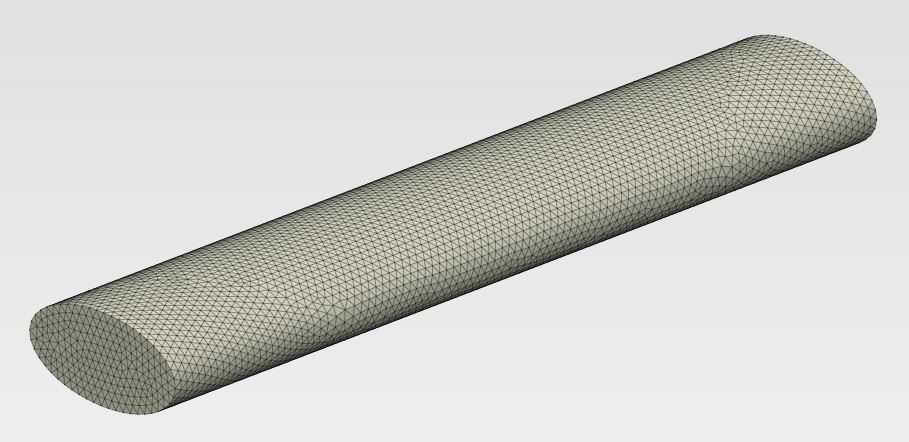
\includegraphics[width=127mm]{fig/03-01.png}
	\caption{楕円形の棒 - メッシュ}
	\label{fig:03-01}
	\end{figure}
\item
  新しい材料を定義し、弾性挙動を加え、ヤング率を210000MPa、ポアソン比を0.3と指定します。
  先に作成した材料を参照して新しいソリッドセクションを作成し、そのセクションがこのパーツに割り当てられるようにシャフトを選択します。
\item
  座標(0, 0, 1000)に基準点を作成します。
  この基準点を使って剛体拘束を作成し、シャフトの表面に割り当てます。
\item
  デフォルトの設定で静的解析ステップを定義します。
  固定境界条件を基準点のある面と反対側のシャフトの面に割り当てます。
  モーメント荷重を作成して基準点に適用し、棒の軸に1000000Nmmの大きさを指定します(図\ref{fig:03-02})。
	\begin{figure}[H]
	\centering
	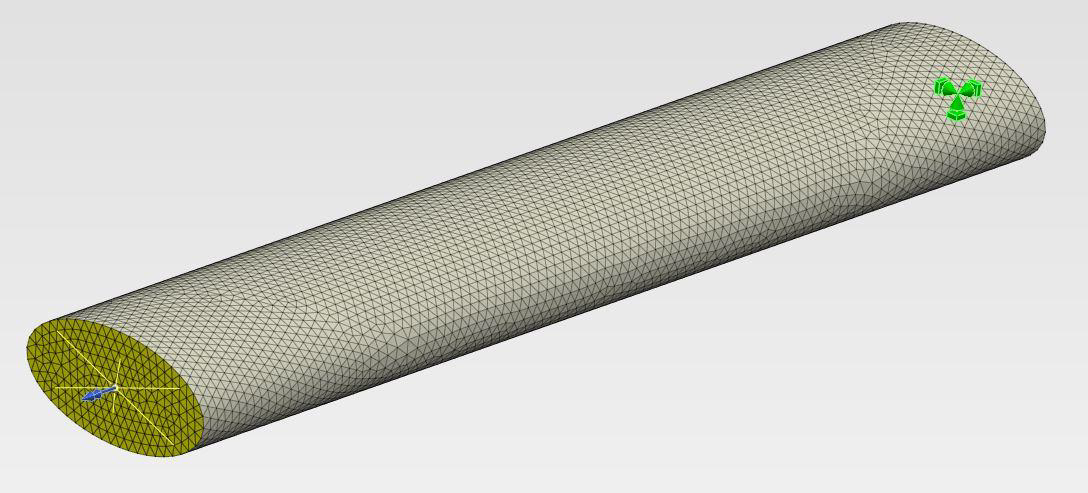
\includegraphics[width=142mm]{fig/03-02.png}
	\caption{楕円形の棒 - 境界条件と荷重}
	\label{fig:03-02}
	\end{figure}
\item
  解析を実行し、解析が完了したら結果を開きます。
  このケースでは、分析的に計算された最大せん断応力は2.547MPaです。
  数値結果と比較するために、適切な応力成分に切り替えます(モデルがグローバル座標系の軸にどのように配置されているかによって異なります)。
  Query → Point/Nodeツールを使って、棒のさまざまな場所の応力値を調べます。
  また、最大せん断応力を持つノードを指すラベルを表示します。
  この場合の結果は2.555MPaで、解析解に非常に近いものでした(図\ref{fig:03-03})。
	\begin{figure}[H]
	\centering
	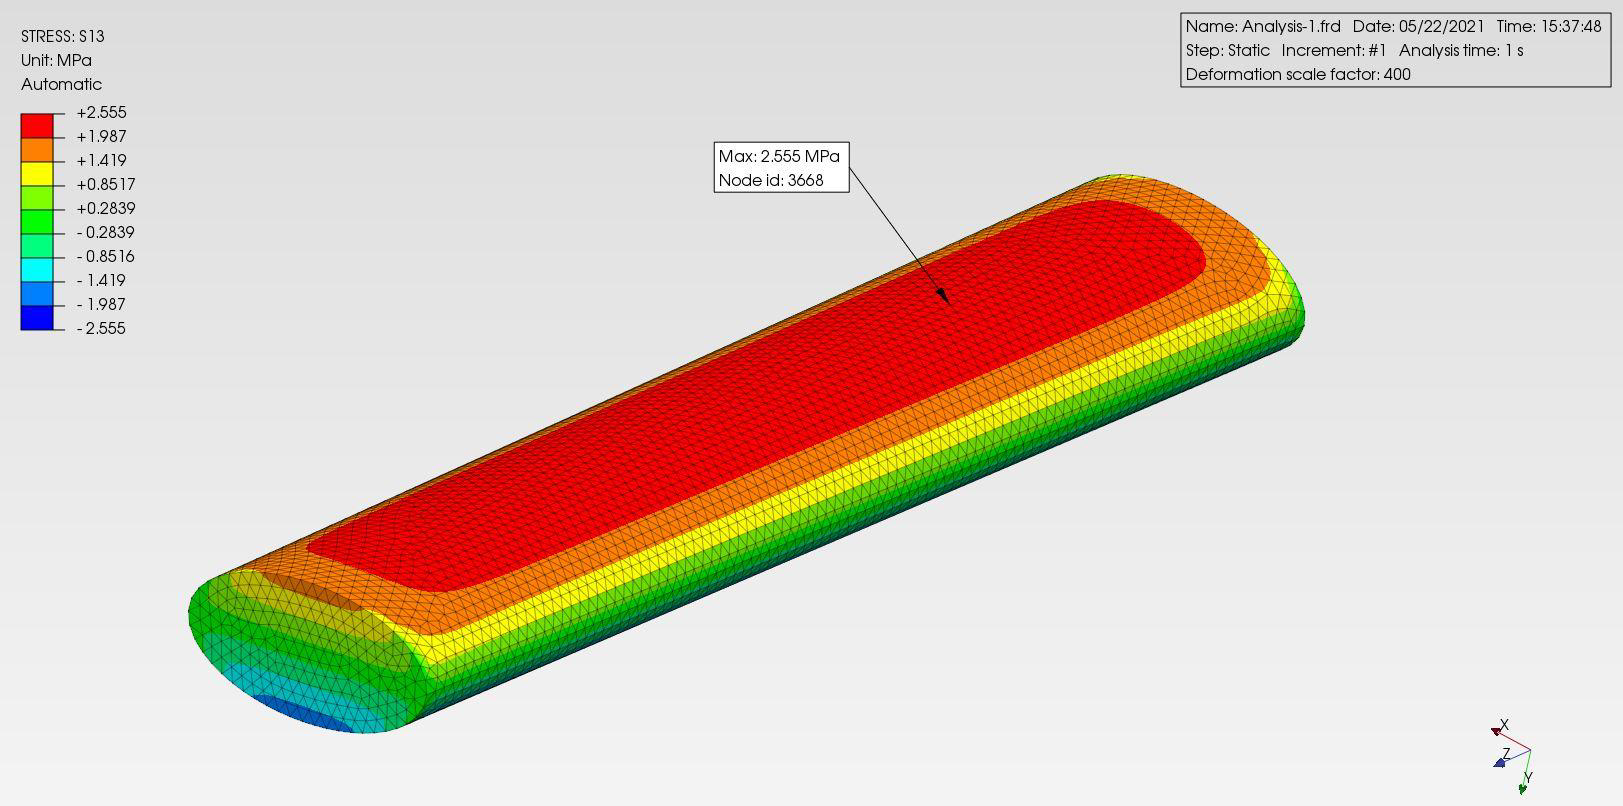
\includegraphics[width=150mm]{fig/03-03.png}
	\caption{楕円形の棒 - せん断応力}
	\label{fig:03-03}
	\end{figure}
\end{enumerate}